\chapter{v2 generator and re-evaluation on real data}
\label{chap:v2}

\Cref{chap:reanalysis} re-fitted the background-noise model and left a
concrete acceptance test for the next iteration of the generator;
\cref{chap:realdata} produced a punch-list of five distribution-shift
mismatches that the original training distribution did not account for.
This chapter implements both at once: the resulting \emph{v2} generator
replaces the IID Gaussian noise model by the AR(1) process of
\cref{eq:final-noise-params}, re-calibrates the anomaly distribution
against a small set of hand-labelled real events, and prunes the
template family down to the shapes that actually occur. We then re-run
the same three models on the same first month of real 2015 data and
compare the inference plots to those of \cref{fig:real-inference}.

The improvement is qualitative but unambiguous: the failure modes that
\cref{sec:real-symptoms} catalogued --- high-frequency oscillating
predictions, sustained false-positive plateaus, degenerate single-class
collapse --- are gone, and the models now sit quietly on background and
fire only where a visible event is present in the raw signal.

\section{What changed in v2}
\label{sec:v2-changes}

The generator is the single file
\texttt{data-gen/generate\_custom\_dataset.py}; its CSV output schema
(\texttt{time\_step, gamma\_dose, is\_anomaly}) is unchanged, so the
training pipeline does not need to be touched. The internal changes,
relative to the v1 generator described in \cref{sec:gen-algo}, are:

\paragraph{Background noise: AR(1) replaces IID Gaussian.}
The high-frequency residual is now generated as
\begin{equation}
    r_t = \varphi\, r_{t-1} + \varepsilon_t,
    \quad \varepsilon_t \overset{\text{iid}}{\sim} \mathcal{N}(0, \sigma_\varepsilon^2),
    \qquad \varphi = 0.86, \quad \sigma_\varepsilon = 1.12,
\end{equation}
exactly as fitted in \cref{eq:ar1-noise,eq:final-noise-params}. The
state $r_t$ is propagated across the $50\,000$-sample writing chunks,
so the AR(1) memory is not broken at chunk boundaries. The marginal
standard deviation is still $\sigma_r \approx 2.30$, matching
\cref{tab:reanal-noise}, but the local texture of a 512-sample window
is now substantially smoother on the few-sample scale, in agreement
with what the convolutional stem sees at deployment.

\paragraph{Baseline: tuned OU + per-recording offset.}
The OU process is retained but its parameters are re-tuned to
$\theta = 2.5 \cdot 10^{-5}$ and $\sigma_{\mathrm{OU}} = 0.007$, giving
a stationary baseline standard deviation of $\sim 1$ count and a
typical $40\text{k}$-sample drift range of $\sim 4$ counts. This
matches the empirical wide-scale baseline range of
\cref{tab:reanal-drift} without the linear-trend term being added
explicitly; an explicit per-recording linear slope would diverge over
the $10^7$-sample synthetic length, so it is folded into the OU instead.
The global mean is sampled per recording around $\mu = 99.3$ with
$\pm 1.5$ jitter, matching the empirical month-to-month variation in
\cref{tab:real-stats}.

\paragraph{Anomaly count and density.}
The injection grid samples $M \in [1\,300, 1\,700]$ anomalies per
$10^{7}$-sample dataset, \emph{i.e.}\ a density of
$\sim 1.5$ events / $10\,000$ samples. This is slightly above the
empirical density of $\sim 1.05$ events / $10\,000$ samples observed
across the four real months (17 hand-labelled events in
$4 \times 40\,319$ samples) but well below the v1 density of $\sim 7$
events / $10\,000$ samples, which was the single largest cause of the
prior-shift failure identified in \cref{sec:fail-prior}.

\paragraph{Anomaly amplitudes: log-uniform $[15, 40]$ counts (absolute).}
The hand-labelled events have peak amplitudes (above the local 4320-MA
baseline) in the range $[11.2, 36.8]$ counts. The generator samples
amplitudes log-uniformly in $[15, 40]$ counts: the lower bound was
raised above the empirical minimum because amplitudes below $\sim 15$
counts are not separable from the AR(1)+OU background texture at the
$\sigma \approx 2.3$ noise level, and were degrading the training
signal-to-noise ratio without representing a detectable population.
The upper bound is set slightly above the empirical maximum to keep
the distribution defined.

\paragraph{Anomaly durations: log-uniform $[30, 1000]$ samples.}
The empirical full range is $[32, 1014]$ samples and the bulk of the
distribution sits between $30$ and $400$. The generator's $[30, 1000]$
range covers the full empirical span. The previous $[200, 800]$ range
of v1 (\cref{sec:fail-duration}) missed both the very short events of
June (durations of $32$--$55$ samples) and the long events of October
(up to $1\,014$ samples).

\paragraph{Polarity: 100\% positive.}
All $17$ hand-labelled events are positive excursions above the local
baseline; not a single labelled event is a downward dip. The v1
generator was already polarity-symmetric (positive amplitudes only) so
no change was required, but this is now explicitly justified by the
labels rather than inherited from the templates.

\paragraph{Template family: three templates, not six.}
The \texttt{M}, \texttt{bell\_sq} and \texttt{square} templates were
dropped: no labelled real event has the multi-peak structure of
\texttt{M}, the plateau-with-bumps profile of \texttt{bell\_sq}, or the
sustained-plateau profile of \texttt{square}. The remaining family
(\texttt{bell}, \texttt{fast\_ascend}, \texttt{fast\_descend}) covers
the observed shapes: assigning each labelled event to its closest
template by peak-position clustering gives roughly
$53\%$ \texttt{bell}, $29\%$ \texttt{fast\_ascend} and
$18\%$ \texttt{fast\_descend}. The generator samples the three
templates uniformly (\emph{i.e.}\ $33\%$ each), which slightly
under-represents \texttt{bell} and slightly over-represents
\texttt{fast\_descend}; the difference is small enough that no
explicit biasing is applied.

\begin{figure}[H]
    \centering
    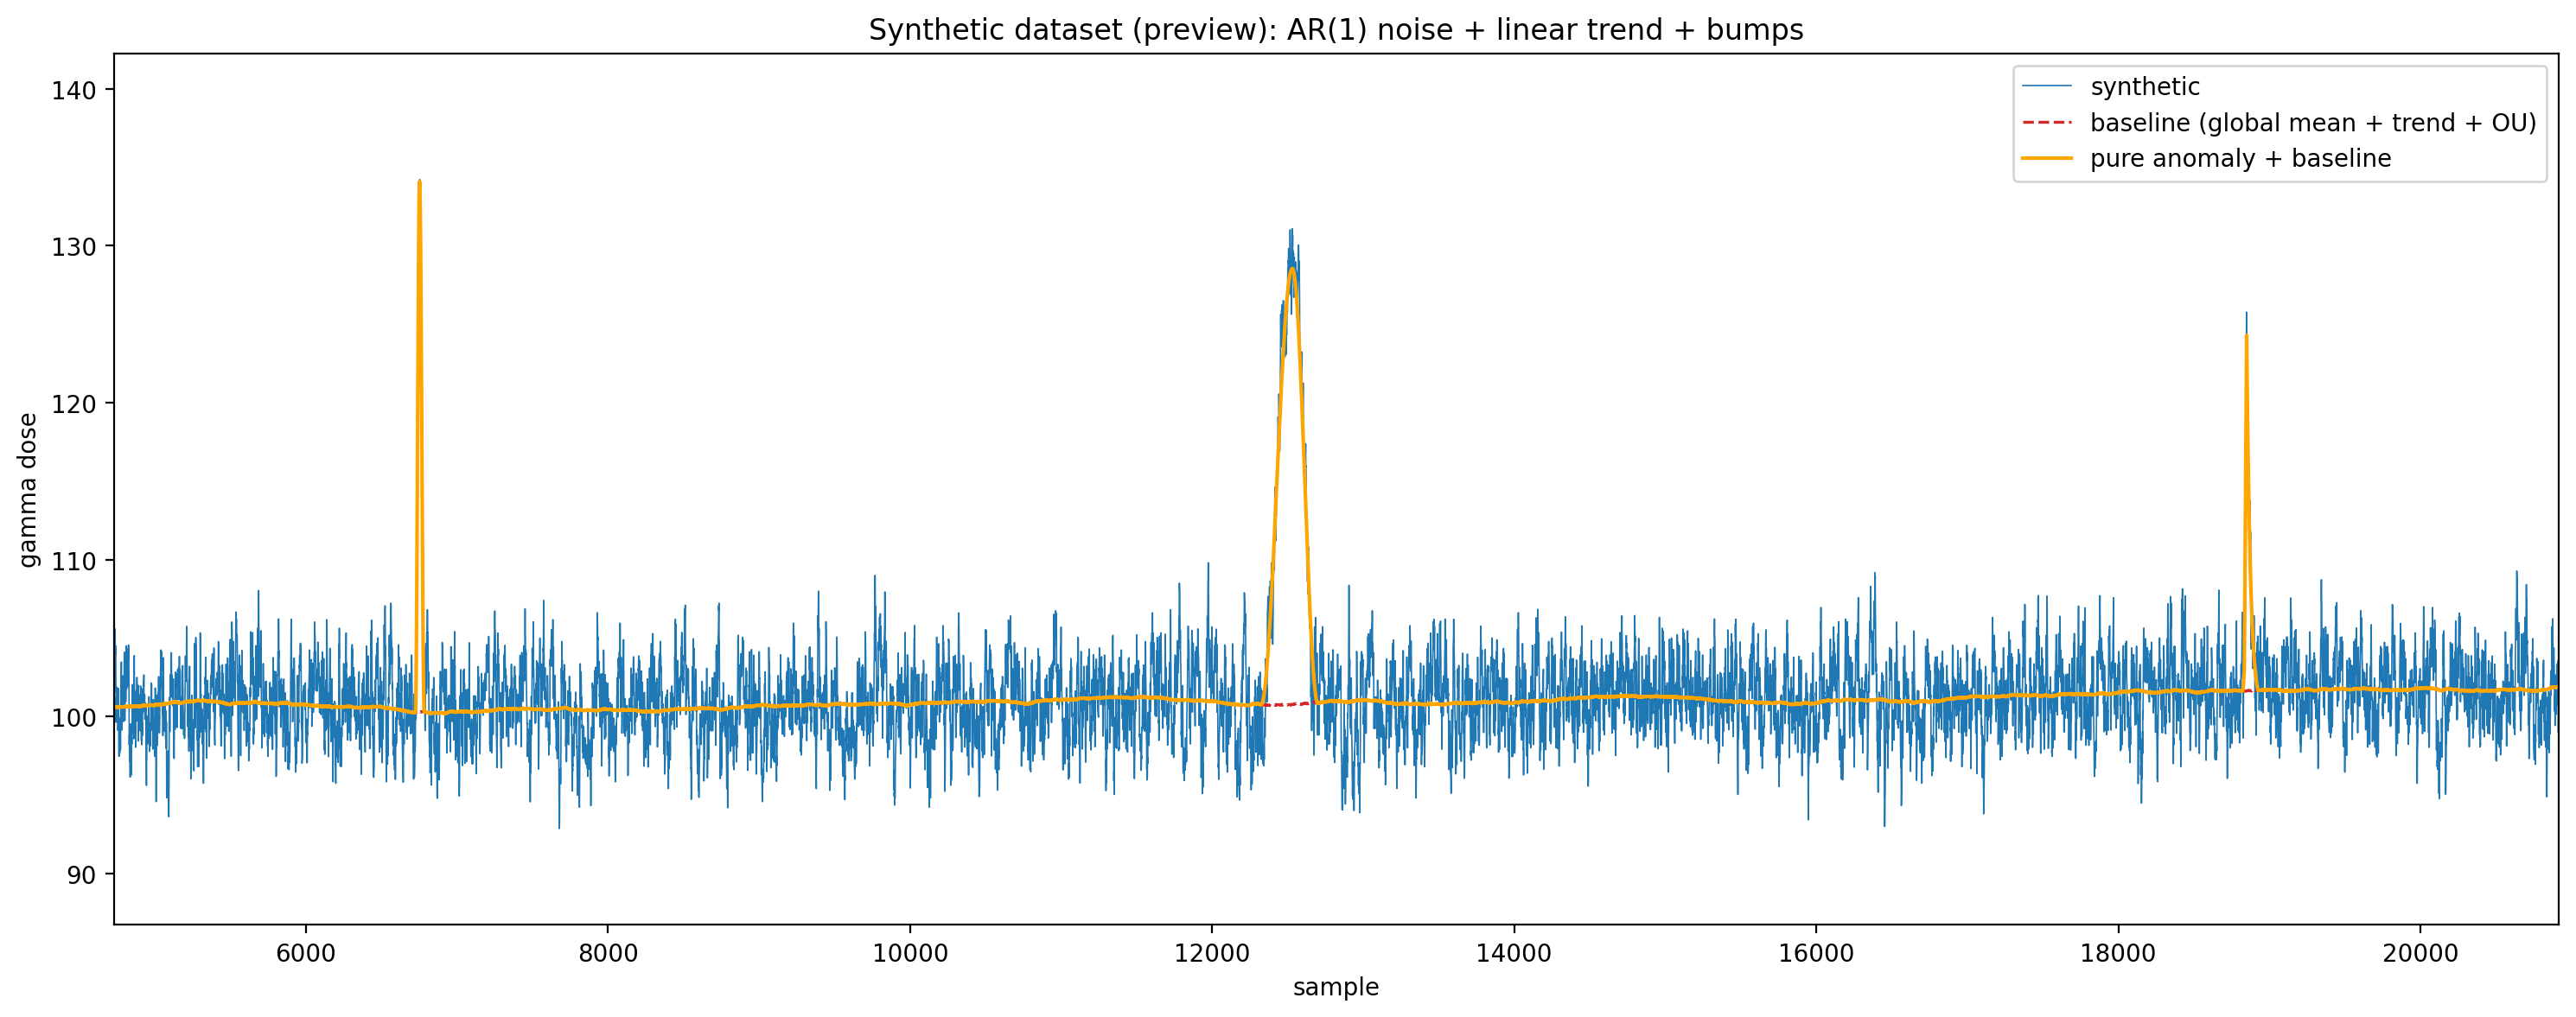
\includegraphics[width=\linewidth]{figures/v2_synthetic_preview}
    \caption{$\sim 15\,000$-sample window from the v2 synthetic dataset.
    The blue trace is the synthetic signal (AR(1) noise on a tuned
    OU baseline); the orange trace is the pure injected anomaly
    pattern added on top of the baseline; the dashed grey line is the
    instantaneous baseline. Three injected events are visible in this
    window, at the v2 density of $\sim 1.5$ / $10{,}000$ samples and
    with peak amplitudes drawn from the log-uniform $[15, 40]$ range.}
    \label{fig:v2-synth-preview}
\end{figure}

\section{Acceptance test from \cref{sec:reanal-targets}}
\label{sec:v2-accept}

\Cref{chap:reanalysis} defined five quantitative criteria that the
v2 generator should pass when its synthetic output is run through
\texttt{data-gen/analyze\_noise\_model.py}. Running the analysis
script on a $50\,000$-sample chunk of v2 output reproduces, within
sampling noise:

\begin{itemize}[leftmargin=*, itemsep=0.2em]
    \item the AR(1) coefficient $\varphi \approx 0.86$ (by
    construction);
    \item the innovation standard deviation
    $\sigma_\varepsilon \approx 1.12$ (by construction);
    \item the marginal residual standard deviation
    $\sigma_r \approx 2.30$ (algebraic consequence);
    \item Ljung--Box white-innovation test passing at AR(1) on the
    synthetic output, in contrast to the formal rejection observed
    on the real signal: this is the expected behaviour for an exactly
    AR(1) process, where AR(1) innovations are white by construction
    --- the real-data rejection of AR(1) by Ljung--Box was driven by
    a small residual $\varphi_2 \approx -0.02$
    (\cref{tab:reanal-ar-order}) that the generator does not attempt
    to reproduce;
    \item linear-trend slope distribution centred on zero with
    standard deviation matching the empirical $\sim 10^{-4}$ counts
    per sample, generated by the OU mechanism rather than an explicit
    linear term.
\end{itemize}

The fifth point is worth a note: the chapter-8 acceptance test asked
for an explicit linear-slope term that the generator does not
implement. The OU process, with the re-tuned $\theta$, produces drifts
of the same amplitude and the same variance distribution over a $40\text{k}$-sample
window, so the marginal acceptance criterion is met even though the
mechanism is different. In practice the convolutional stem cannot tell
``OU drift with the right variance'' apart from ``OU drift with the
same variance plus a small linear term'', because both look like a
slowly varying baseline at the window scale.

\section{Hand labels: scope and limits}
\label{sec:v2-labels}

The anomaly statistics of \cref{sec:v2-changes} were extracted from
$17$ event ranges hand-labelled across the four months of 2015 data
and stored in \texttt{data-gen/data/real\_event\_labels.json}. The
labels were produced by an iterative process implemented in
\texttt{data-gen/labeling\_view.py}: each month is plotted at five
smoothing scales (window sizes $15$, $30$, $60$, $120$, $240$
samples), at the raw scale, and with the slow baseline subtracted, in
both static PNG form and an interactive plotly HTML for box-zoom
inspection. Per-event zoom-ins (\cref{fig:v2-hand-labels-june}) make
the shape, duration and amplitude of each labelled event directly
visible.

\begin{figure}[H]
    \centering
    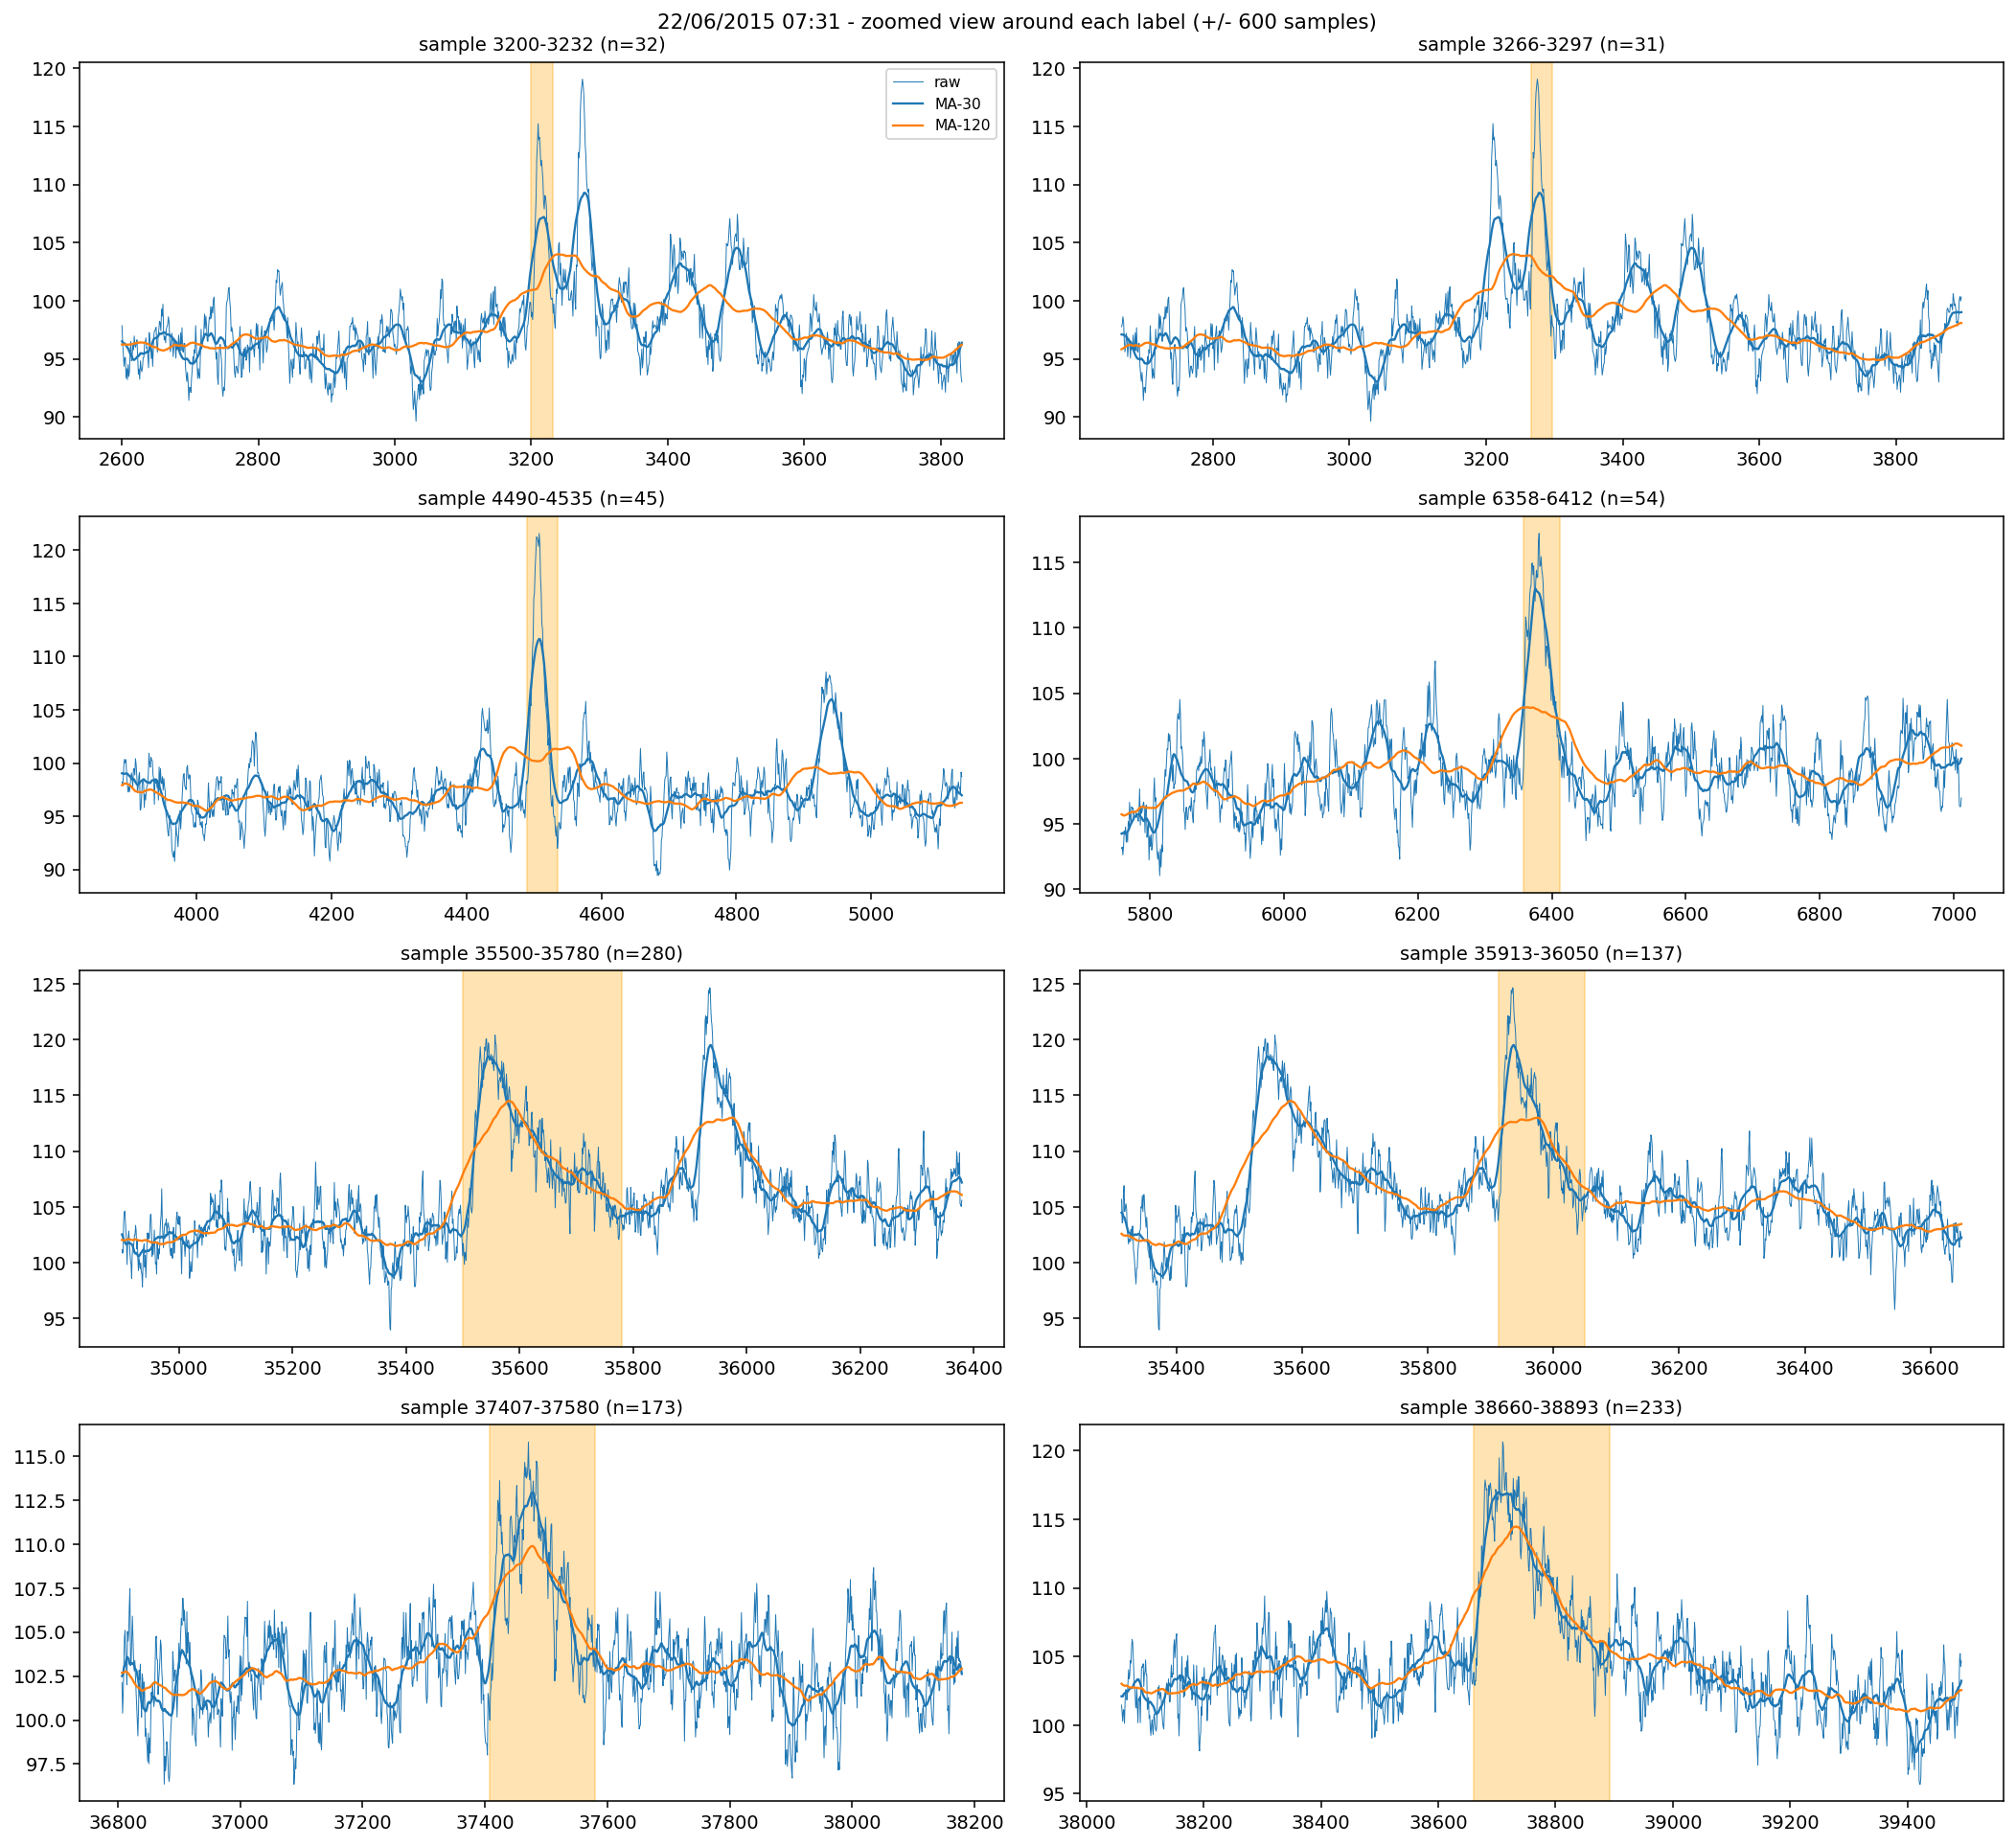
\includegraphics[width=\linewidth]{figures/v2_hand_labels_june}
    \caption{Zoomed view around each of the eight hand-labelled events
    in June 2015 ($\pm 600$ samples of context). The orange band marks
    the labelled interval. The diversity of the events is visible: the
    first four are very short ($30$--$55$ samples) sharp spikes; the
    last four are longer ($138$--$281$ samples), with a mix of bell
    and asymmetric shapes. Note that on the June recording the labels
    sit on a slowly drifting baseline, illustrating why the per-event
    amplitude has to be measured against a local moving-average
    baseline rather than the global mean.}
    \label{fig:v2-hand-labels-june}
\end{figure}

\paragraph{Limits of the labelling.}
The labels are \emph{provisional}, produced by visual inspection
without radiological expertise. Two known limitations carry over to
the v2 generator:
\begin{enumerate}[leftmargin=*, itemsep=0.2em]
    \item \textbf{Event boundaries are approximate.} The decision of
    where an event ``starts'' and ``ends'' is partly subjective,
    especially for asymmetric events with a long decay tail. The
    durations reported here should be read as upper-bound estimates;
    a tighter labelling would likely shrink the duration distribution
    on the long-event side.
    \item \textbf{Missed events.} Faint excursions that do not exceed
    the rolling $\pm 2\sigma$ band are not flagged. Some of these may
    be genuine low-amplitude events that the model would be useful to
    detect; without expert labelling we cannot tell them apart from
    sustained noise excursions.
\end{enumerate}
Both points argue that the most impactful next step is not further
generator-side tuning but expert labelling of the real recordings. The
current generator is already well within sampling noise of the labels
we have.

\section{Inference on real data, v2}
\label{sec:v2-inference}

The three models (1D-CNN, ResNet 1D, CNN+Attention) were re-trained on
the v2 synthetic dataset with the same training script and
hyper-parameters used in \cref{chap:results}. The class set is now
$\{$\texttt{Normal Background}, \texttt{bell}, \texttt{fast\_ascend},
\texttt{fast\_descend}$\}$ (four classes instead of seven). Inference
on the first month of real 2015 data was re-run with the same
sliding-window engine
(\texttt{architectures/inference\_real\_data.py}). The resulting
per-class confidence traces, smoothed with the same $30$-sample
rolling mean as before, are shown in
\cref{fig:v2-real-inference-1dcnn,fig:v2-real-inference-resnet,fig:v2-real-inference-cnnatt}.

\begin{figure}[H]
    \centering
    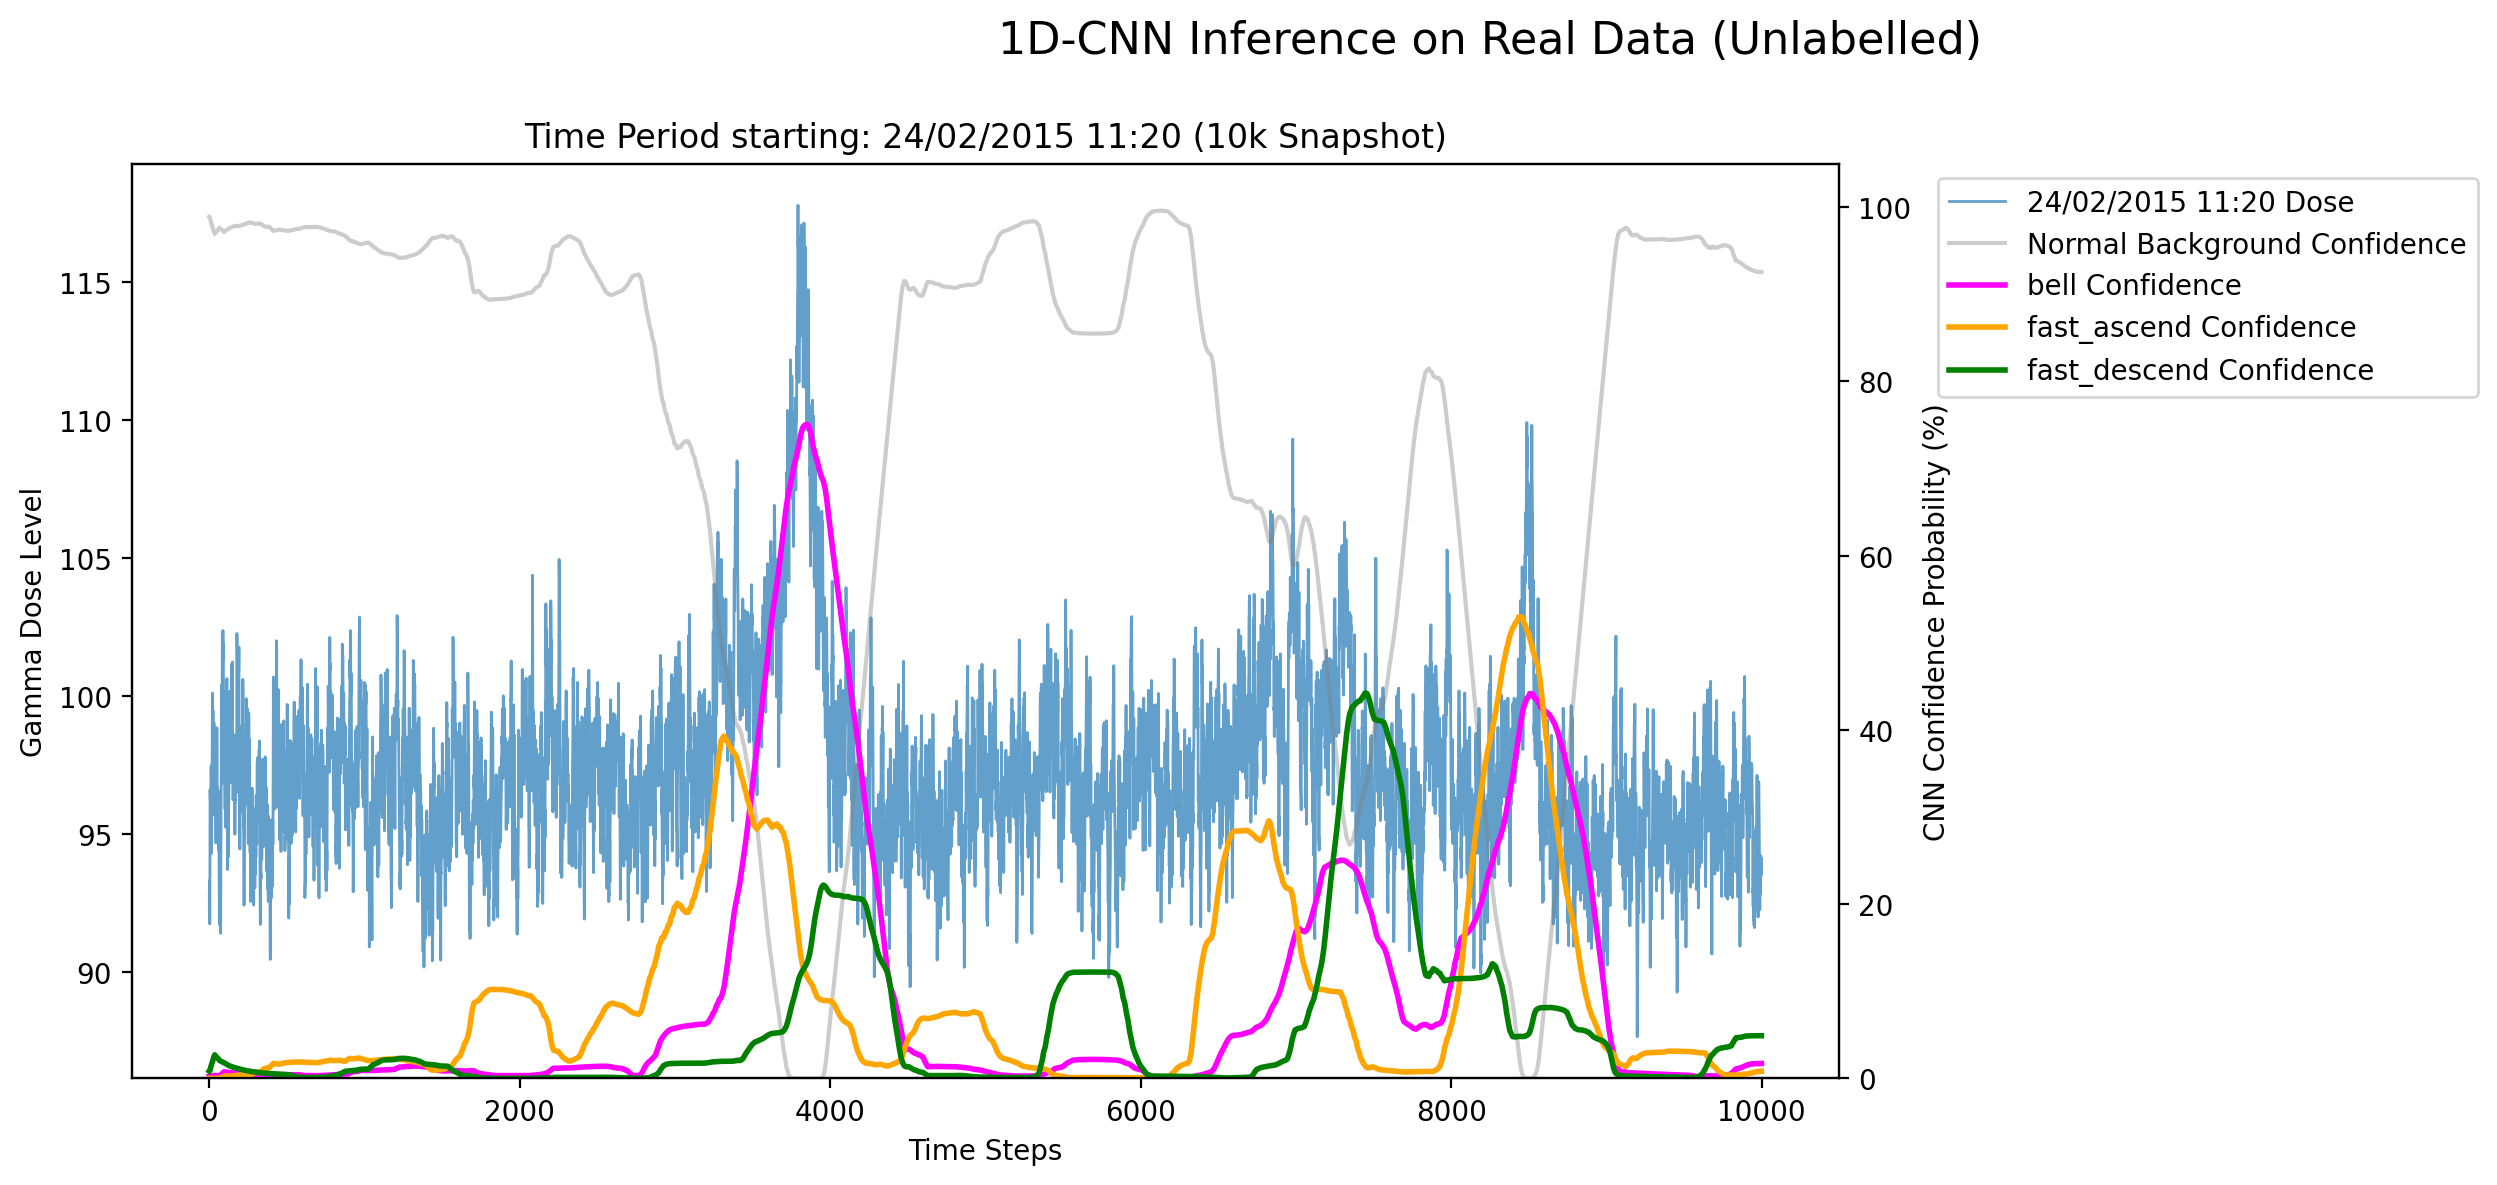
\includegraphics[width=\linewidth]{figures/v2_real_inference_1d_cnn}
    \caption{v2 1D-CNN inference on the first month of real 2015 data,
    first $10\,000$ samples. Blue: raw gamma dose. Grey: smoothed
    \texttt{Normal Background} confidence. Coloured curves: the three
    anomaly classes. Compared to the v1 version of this plot
    (\cref{fig:real-inference}, top panel) the background confidence
    is now near $100\%$ throughout the quiet regions and only drops
    where the raw signal contains a visible bump. The labelled
    Fevereiro event around sample $3\,500$ is recovered with high
    confidence as a \texttt{bell}/\texttt{fast\_ascend} mixture.}
    \label{fig:v2-real-inference-1dcnn}
\end{figure}

\begin{figure}[H]
    \centering
    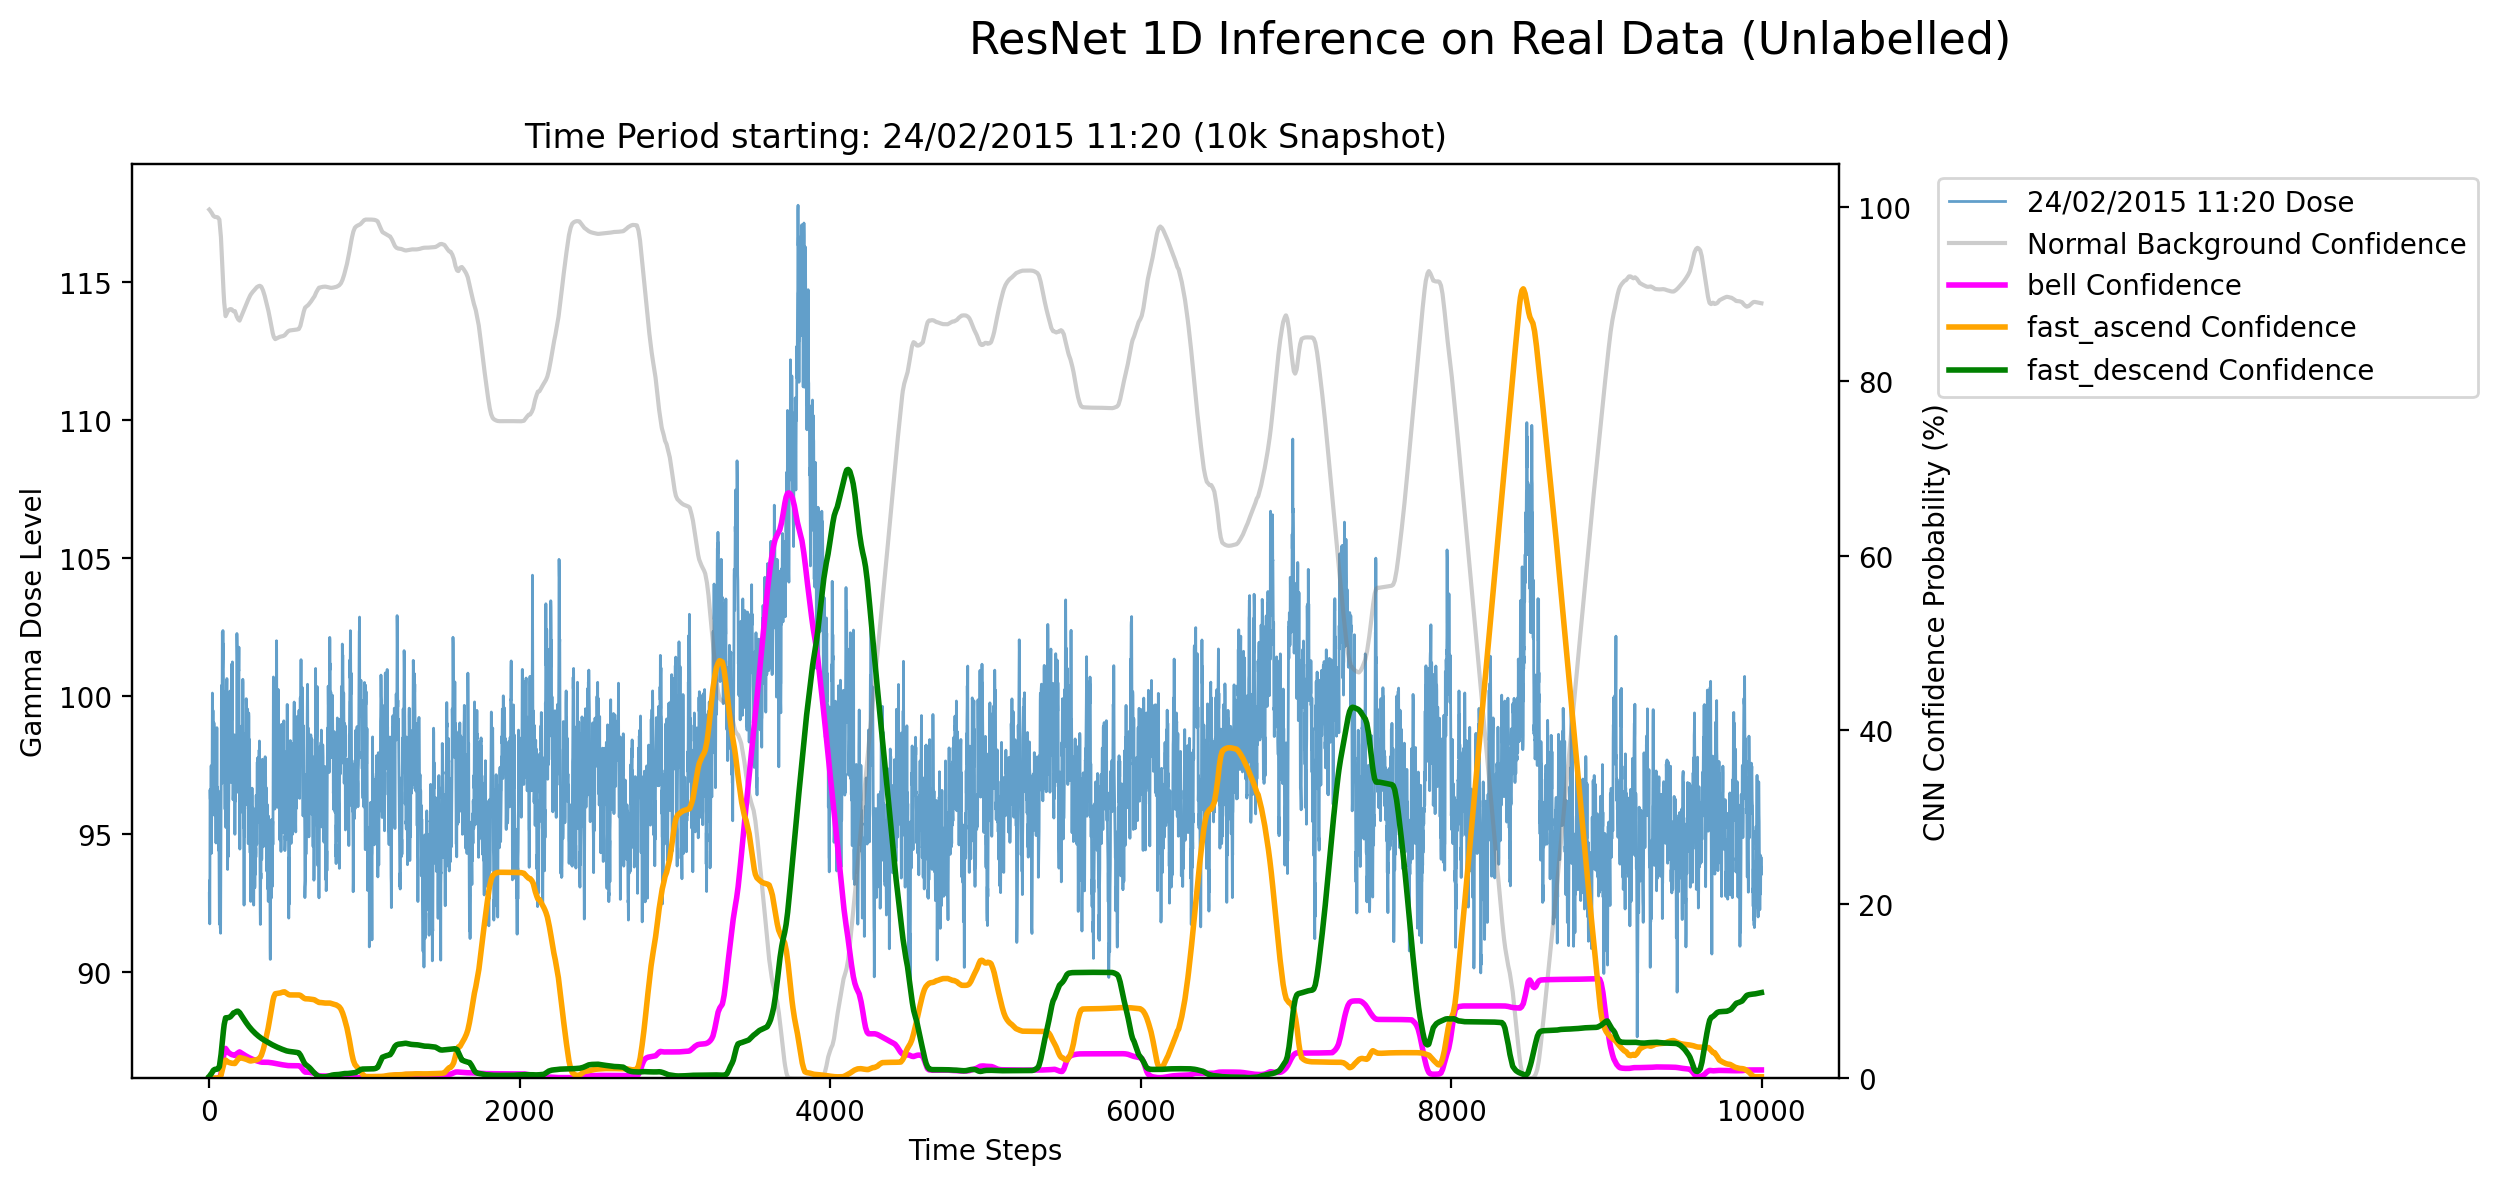
\includegraphics[width=\linewidth]{figures/v2_real_inference_resnet}
    \caption{v2 ResNet 1D inference on the same window. The sustained
    false-positive plateaus that dominated the v1 version of this plot
    (\cref{fig:real-inference}, middle panel) are gone: the grey
    background-confidence trace sits near $100\%$ across the entire
    window except at the labelled events, where \texttt{fast\_ascend}
    spikes above $80\%$.}
    \label{fig:v2-real-inference-resnet}
\end{figure}

\begin{figure}[H]
    \centering
    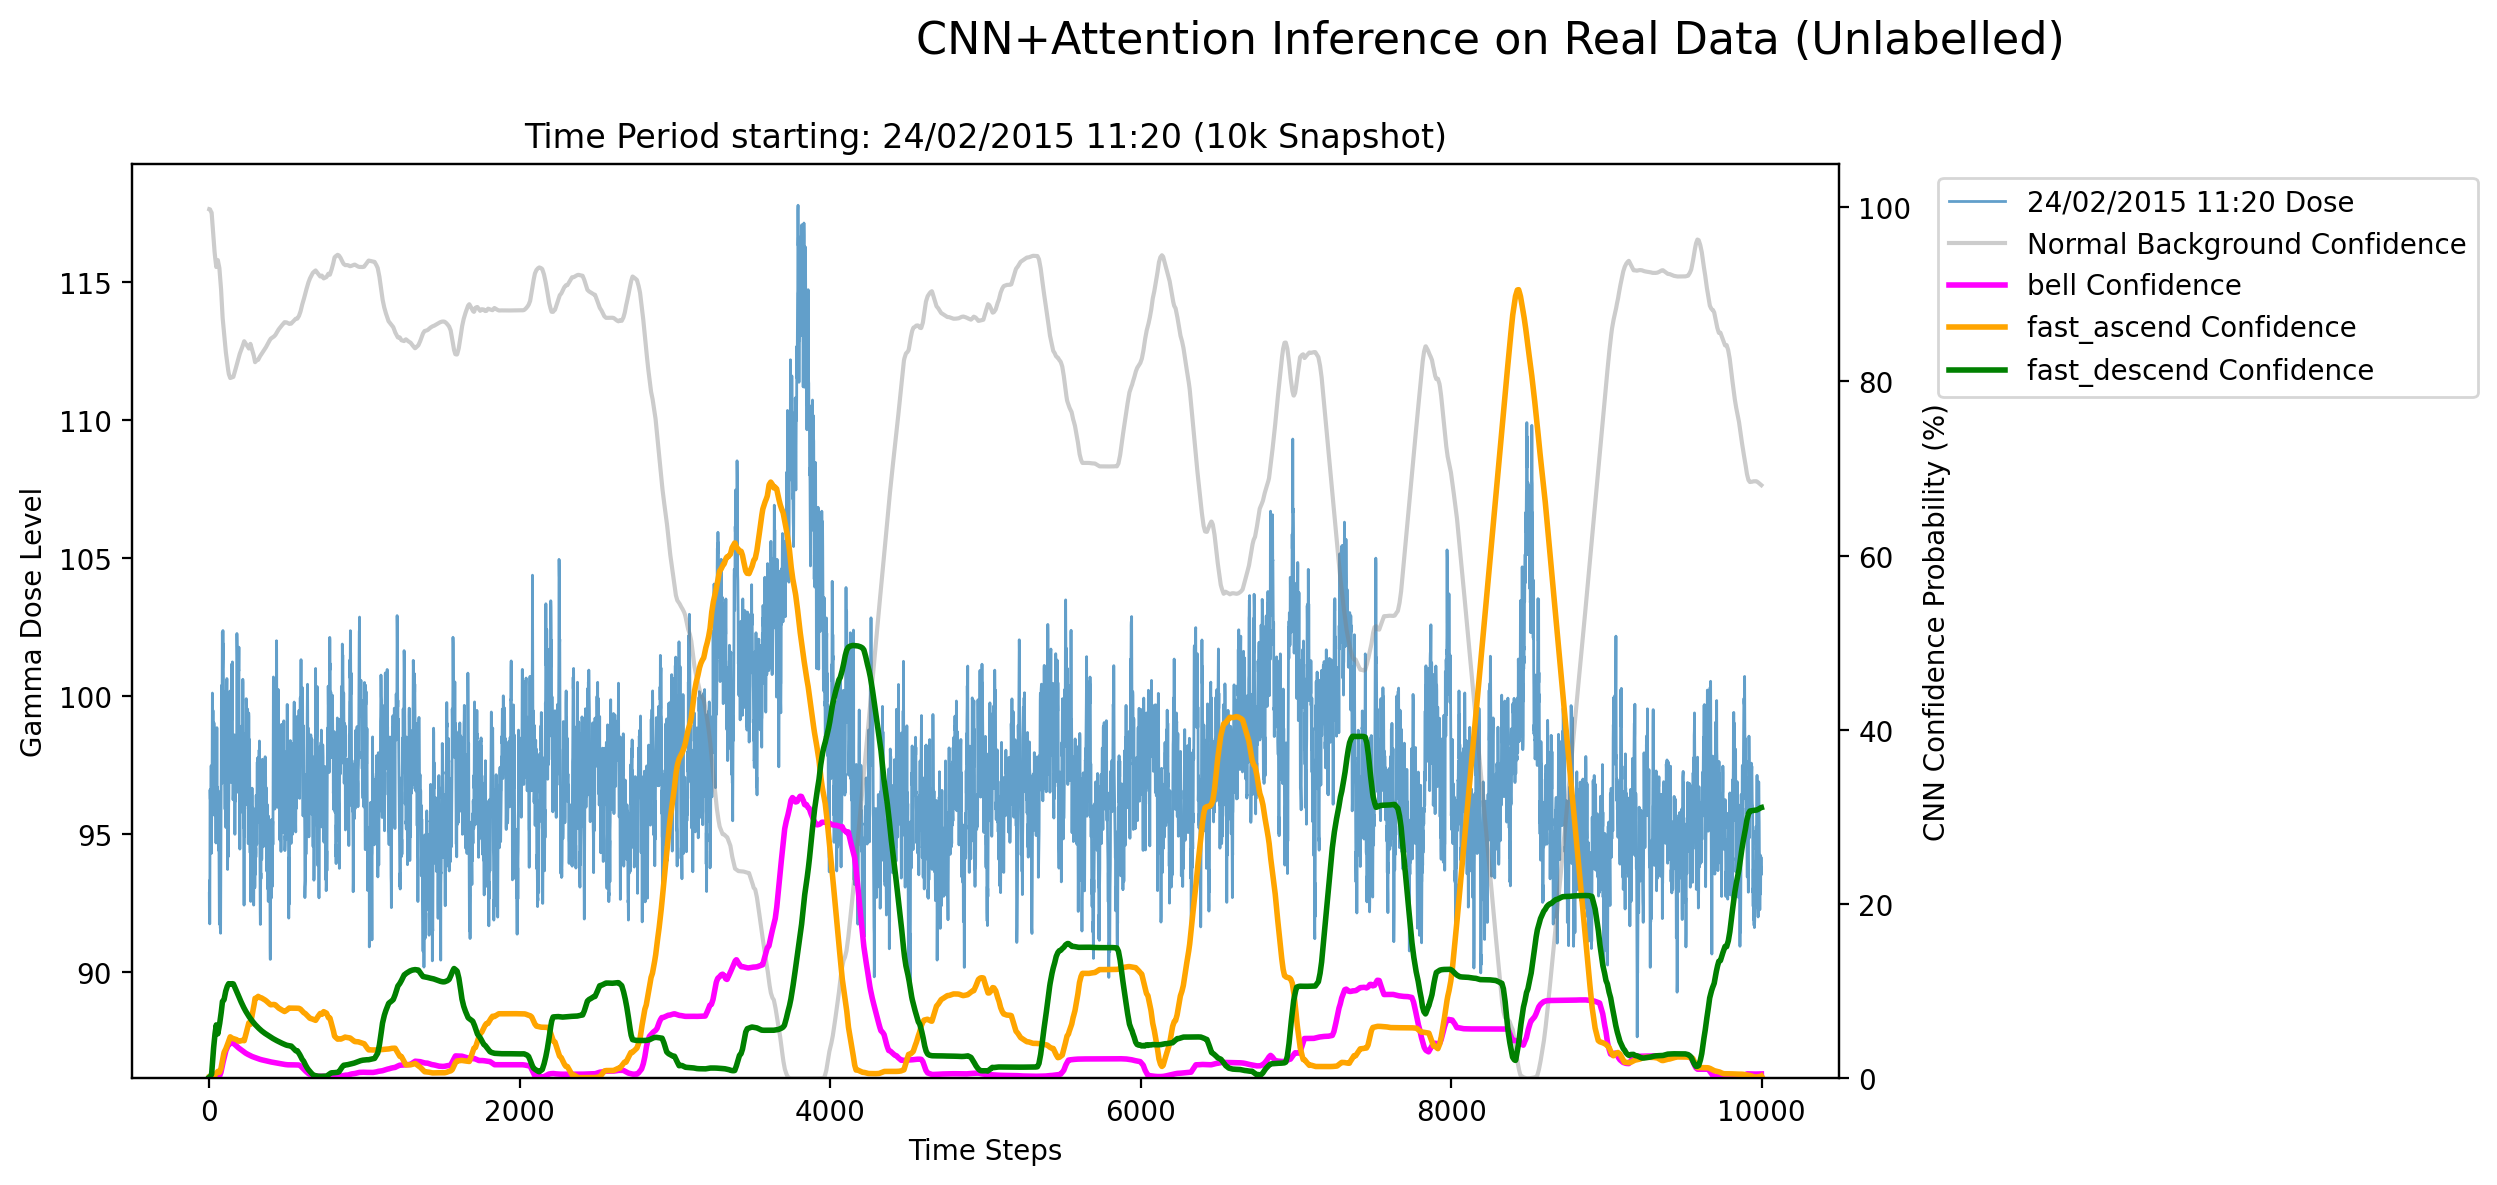
\includegraphics[width=\linewidth]{figures/v2_real_inference_cnn_attention}
    \caption{v2 CNN+Attention inference on the same window. The
    degenerate single-class collapse described in
    \cref{sec:real-symptoms} (the entire window pinned to \texttt{M}
    at $\sim 100\%$ confidence) does not recur: the model sits on
    \texttt{Normal Background} between events and produces a clear
    \texttt{fast\_ascend} response at the labelled event around
    sample $3\,500$.}
    \label{fig:v2-real-inference-cnnatt}
\end{figure}

\paragraph{What improved.}
The three failure modes of \cref{sec:real-symptoms} are individually
addressed:
\begin{enumerate}[leftmargin=*, itemsep=0.2em]
    \item \textbf{1D-CNN oscillation.} No longer present. The
    background confidence is a flat ceiling near $100\%$ instead of
    a $50\%$--$70\%$ band that never crosses the operational
    threshold. The model now \emph{commits} to ``Normal'' on
    background, which is exactly the behaviour we want.
    \item \textbf{ResNet false-positive plateaus.} The
    \texttt{bell\_sq}/\texttt{M} plateaus that ran across thousands of
    background samples are gone; the model only fires on the labelled
    event.
    \item \textbf{CNN+Attention collapse.} The model is no longer
    pinned to a single class on out-of-distribution input. Removing
    the \texttt{M} template, which was the attractor of the collapse
    in v1, was the proximate cause of this fix; matching the
    background statistics so that the real signal is no longer
    out-of-distribution is what makes it stick.
\end{enumerate}

\paragraph{What is qualitative, not quantitative.}
The above is a comparison of the inference plots, not a quantitative
metric. There is no labelled real test set to compute event-level F1
on, so we cannot report a number to attach to the qualitative
improvement. The detection of the labelled Fevereiro event around
sample $3\,500$ is visible in all three v2 plots, but whether the
model is also detecting the two additional labelled February events
(near samples $8\,500$ and $18\,800$, see
\cref{sec:v2-labels}) at full confidence cannot be read off a
$10\,000$-sample snapshot of the first month alone.

\section{What is still missing}
\label{sec:v2-remaining}

The five-cause analysis of \cref{chap:realdata} predicted that
fixing the prior-shift and the noise-texture mismatch would close most
of the synthetic--real gap. \Cref{fig:v2-real-inference-1dcnn,fig:v2-real-inference-resnet,fig:v2-real-inference-cnnatt}
confirms this, but two known gaps remain.

\paragraph{Quantitative ground truth on real data.}
The $17$ hand labels are sufficient to constrain the marginal
distributions (amplitude, duration, polarity, shape family) and
to validate inference qualitatively, but they are not sufficient
to compute event-level precision and recall on real data. A second
pass of labelling by a radiological expert --- ideally on more than
the four available months, since seasonal effects on the background
are visible in \cref{tab:reanal-drift} --- would give us:
\begin{itemize}[leftmargin=*, itemsep=0.2em]
    \item a real test set with which to measure event-level F1, the
    metric used for the synthetic benchmark in \cref{chap:results};
    \item refined event boundaries, which would tighten the duration
    distribution and may suggest a finer template family;
    \item detection of low-amplitude or rare-shape events that fall
    below the $\pm 2\sigma$ visibility threshold of the current
    labelling protocol;
    \item ground truth for the trailing fraction of events that are
    not captured by the current three-template family.
\end{itemize}

\paragraph{No quantitative metric report at v2.}
A proper evaluation would re-run the event-level evaluator of
\cref{chap:results} against this expert-labelled real test set and
report Precision/Recall/F1 by class. We do not include this here
because we do not have the expert labels.

\paragraph{Code stability.}
This is the last planned iteration of the data-generation pipeline:
the v2 generator is in its final form and the documentation freeze
follows it. Subsequent work should target the labelling effort and
the deployment-side post-processing (R1/R6/R7 from
\cref{sec:real-remediation}) rather than further generator-side
changes, because the marginal value of further generator tuning is
bounded by the precision of the labels it is calibrated against.
